\chapter{Предел последовательности}
\section{Определение}
Пусть имеется последовательность $a_n$. Тогда если начиная с некоторго элемента под индексом $N$ каждый следующий элемент $a_n,$ где $n>N$ будет входить в $\varepsilon$-окрестность некоторой точки $A$, то говорят, что последовательность имеет предел и он равен $A$. \newline
$\forall \varepsilon > 0\ \exists N \in \mathbb{N} : \forall n > N(n \in \mathbb{N}),\ a_n \in \mathring{U_\varepsilon}(A)$
\begin{example}
Возьмём $\displaystyle \lim_{n \to +\infty}\frac{(-1)^n}{n} = 0$
\newline
Тут $A = 0$, $a_n = \frac{(-1)^n}{n}$
\newline
Подставим значения в определение:
\begin{center}$\forall\varepsilon > 0\ \exists N \in \mathbb{N} : \forall n > N(n \in \mathbb{N}),\ \frac{(-1)^n}{n} \in \mathring{U_\varepsilon}(0)$\end{center}
$\frac{(-1)^n}{n} \in \mathring{U_\varepsilon}(0) \equiv |\frac{(-1)^n}{n} - 0| < \varepsilon$, т.к. последовательность $a_n$, принадлежащая $\varepsilon$-окрестности в точке $A = 0$ тоже самое, когда расстояние между рассматриваемыми членами $a_n$ и $A = 0$ меньше $\varepsilon$.\newline
Упростим: $|\frac{(-1)^n}{n} - 0| < \varepsilon \Rightarrow |\frac{(-1)^n}{n}| < \varepsilon \Rightarrow \frac{1}{n} < \varepsilon \Rightarrow n > \frac{1}{\varepsilon} $. \newline
1)Возьмём $\varepsilon = \frac{1}{2} \Rightarrow n > 2$. Подставим в формулу наименьшее удовлетворяющее условию $n > 2$ число: $|\frac{-1^3}{3} - 0| = \frac{1}{3}$. Получается, что $\frac{1}{3} < \frac{1}{2}$ и $\forall n > 2: |\frac{(-1)^n}{n} - 0| < \varepsilon$ $\Rightarrow$ все условия из определения соблюдены. \newline
\end{example}

\begin{mydef}Последовательность -- \textbf{сходящеяся}, если она имеет предел.\end{mydef}
\begin{mydef}Последовательность -- \textbf{расходящеяся}, если у нее нет предела\end{mydef}
\begin{mydef}Последовательность называется \textbf{ограниченной}, если все её члены по модулю не превосходят некоторого числа.\end{mydef}

\section{Теорема об единственности предела}
\begin{theorem}
Если последовательность имеет предел, то он единственный.\newline
$\begin{cases}\displaystyle \lim_{n \to +\infty} a_n = A_1 \\ \displaystyle \lim_{n \to +\infty} a_n = A_2\end{cases}$
$\Longrightarrow$ \qquad $\displaystyle A_1 = A_2$
\end{theorem}
Пойдём от противного. Возьмем какие-либо непересекающиеся окрестности $U_{\varepsilon}(A_1)$ и $V_{\varepsilon}(A_2)$ точек $A_1$ и $A_2$ соответственно, $U_{\varepsilon} \cap V_{\varepsilon} = \varnothing$.\newline
Согласно определению предела вне окрестности $U_{\varepsilon}(A_1)$, в частности в окрестности $V_{\varepsilon}(A_2)$, содержится лишь \textbf{конечное} число членов $\{x_n\}$. Однако точка $A_2$ также является ее пределом, и потому в ее окрестности $V_{\varepsilon}(A_2)$ должны находиться все члены последовательности $\{x_n\}$, начиная с некоторого номера, а следовательно, \textbf{бесконечно} много ее членов. Получилось противоречие, значит $A_1 = A_2$, что и требовалось доказать.

\section[Т. об огр. сход. посл.]{Теорема об ограниченности сходящейся последовательности}
\begin{theorem}
Если последовательность сходится, то она является ограниченной.
\end{theorem}
Пусть есть сходящаяся последовательность $a_n \Rightarrow \exists \displaystyle \lim_{n \to +\infty} a_n = a$. \newline 
Возьмём $\varepsilon = c > 0  \Rightarrow \exists N : \forall n > N, |a_n - a| < ca$ \newline
Избавимся от модуля: 
\begin{center} $-c < a_n - a < c$ \end{center}
\begin{center} $a - c < a_n < a + c$ \end{center}
Исходя из верхнего неравентсва, если взять $max$ из $|a_n|, |a - c|$ и $|a + c|$, причём $n \leq N$
\begin{center} $A = max(|a_n|, n \leq N; |a - c|; |a + c|)$ \end{center}
то получится, что $|a_n| \leq A, \ \forall n \in \mathbb{N}$, что и требовалось доказать.

\section[Т. о пред. перех. в нерав.]{Теорема о предельном переходе в неравенстве}
\begin{theorem}
Пусть заданы две последовательности ${a_n}$и ${b_n}$. Если $\displaystyle \lim_{n \to +\infty} a_n = a, \displaystyle \lim_{n \to +\infty} b_n = b$, и начиная с некоторого номера $a_n \leq b_n$, то выполняется неравенство $a \leq b$.  \newline
$\begin{cases}
\displaystyle \lim_{n \to +\infty} a_n = a \\ \displaystyle \lim_{n \to +\infty} b_n = b
\\ \forall n > N, a_n \leq b_n
\end{cases}$
$\Longrightarrow$ \qquad $\displaystyle a \leq b$
\end{theorem}
Докажем от противного. Пусть $a > b$, $\varepsilon = \frac{a - b}{2}$. Скажем, что
\begin{center}
$\exists N_a: \forall n > N_a, |a_n - a| < \varepsilon$
\end{center}
\begin{center}
$\exists N_b: \forall n > N_b, |b_n - b| < \varepsilon$
\end{center}
Возьмём максимальный номер $N = max(N_a, N_b)$ и тогда получится, что $\forall n > N$ верно:
\begin{center}
$a - \varepsilon < a_n < a + \varepsilon$
\end{center}
\begin{center}
$b - \varepsilon < b_n < b + \varepsilon$
\end{center}
 \begin{center}
  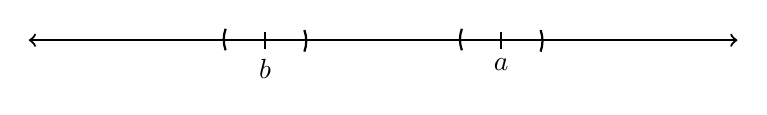
\begin{tikzpicture}[thick]
    \draw[thick, <->](0.5,0)--(9.5,0);
   \draw[thick,black] (4, -0.145) arc (-20:20:0.4cm);
   \draw[thick,black] (3, 0.145) arc (160:200:0.4cm);
   \draw[thick,black] (7, -0.145) arc (-20:20:0.4cm);
   \draw[thick,black] (6, 0.145) arc (160:200:0.4cm);
    \foreach \x/\xtext in {3.5/$b$, 6.5/$a$}
      \draw(\x,3pt)--(\x,-3pt) node[below] {\xtext};
  \end{tikzpicture}
 \end{center}

Мы знаем, что $a > b$, тогда из верхних неравенств вытекает, что $b_n < a_n$. Получили противоречие, значит теорема верна.



\section[Т. о п/посл. сход. послед.]{Теорема о подпоследовательности сходящейся последовательности}
\begin{theorem}
Если последовательность стремится к $A$, то любая её подпоследовательность тоже стремится к $A$.\newline
$\displaystyle \lim_{x \to +\infty} a_n = A \Rightarrow \forall a_{n_k} \lim_{k \to +\infty} a_{n_k} = A$
\end{theorem}
По определению предела найдётся такой номер, что все члены с б\'oльшими номерами принадлежат $\varepsilon$-окрестности.
$\forall \varepsilon > 0\ \exists N:\ \forall n > N\ |a_n - A| < \varepsilon$\newline
Тогда $\forall k > N:\ \forall n_k > N$,\  $|a_{n_k} - A| < \varepsilon$.\newline
Значит $a_{n_k}$ стремится к $A$ по определению предела для последовательности, что и требовалось доказать.  

\section[Т. о влож. отрезках]{Теорема Коши-Кантора о вложенных отрезках}
\begin{theorem}
Для всякой системы бесконечного числа вложенных отрезков существует хотя бы одна точка, принадлежащая всем отрезкам системы.\newline
$\bigcap\limits_{n=1}^{\infty} [a_n, b_n] = c$\newline
Если длины отрезков стремятся к нулю, то такая точка \textbf{единственна}.
\end{theorem}
Обозначим за $\{ a_n\}$ множество левых концов отрезков, а за $\{ b_m \}$ -- множество правых концов.
Заметим, что $\forall n, m:\ a_n \leq b_m$. Из \textit{аксиомы непрерывности} заключаем существование точки $c$, лежащей между любыми двумя левым и правым концами:\newline
$\forall n, m\ \exists\  c: \quad a_n \leq c \leq b_m$\newline
В частности (когда $n = m$): $a_n \leq c \leq b_n$\newline 
Последнее выражение означает существование точки между концами самого маленького отрезка. Эта точка -- объединение всей системы, что и требовалось доказать.\newline\newline

Докажем единственность этой точки при стремлении длин отрезков к нулю.\newline
Пусть это не так и существуют точки $c_0,\ c_1,\ c_0 \neq c_1$. Тогда из рассуждений предыдущего доказательства следует:\newline
$(1) \quad \forall n:\ \ c_0,\ c_1 \in [a_n, b_n]$ и $|c_1 - c_0| \leq b_n - a_n$.
Т.к. длины отрезков стремятся к нулю:\newline
$(2) \quad \forall \varepsilon > 0:\ \exists N:\ \forall n > N:\ b_n - a_n < \varepsilon$ (по определению предела).\newline
Но если взять $\varepsilon = \frac{1}{2} |c_1 - c_0|$, то из $(1)$ и $(2)$ получим противоречие: $|c_1 - c_0| < \frac{1}{2} |c_1 - c_0|$.\newline
Таким образом точка $c$ единственна в случае стремления длин отрезков к нулю, что и требовалось доказать.

\section[Т. Больцано]{Теорема Больцано — Вейерштрасса}
\begin{theorem}
На любой ограниченной последовательности $x_n, n \in \mathbb{N}$ можно выделить сходящююся подпоследовательность $x_{n_k}, k \in \mathbb{N}$
\end{theorem}
Если последовательность $x_n$ ограниченна, то всё её бесконечное множество членов принадлежит некоторому промежутку, обозначим его -- $[a_0, b_0]$. Разделим этот промежуток на два равных отрезка, тогда хотя бы один из них будет содержать бесконечное число членов последовательности $x_n$, обозначим этот отрезок, как $[a_1, b_1]$. Продолжая процесс получим последовательность вложенных отрезков.
\begin{center}$[a_0, b_0] \supset [a_1, b_1] \supset [a_2, b_2] \supset \ldots$\end{center}
В которой каждый отрезок $[a_{k+1}, b_{k+1}]$ является половиной отрезка $[a_{k}, b_{k}]$ и содержит бесконечное число членов последовательности $x_n$. Т.к. размер отрезка под номером $k$ равен $S_k=\frac{|b_0-a_0|}{2^k}$, то при $k \to +\infty$, $S_k \to 0$. А по лемме о вложенных отрезках, существует единственная точка $\nu$, принадлежащая всем отрезкам.
Тогда выберем подпоследовательность $x_{n_k} \in [a_k, b_k]$. Новая последовательность $x_{n_k}$ будет сходится к точке $\nu$ потому, что и $\nu$, и $x_{n_k}$ принадлежат отрезку $[a_k, b_k]$, размеры которого стремятся к $0$ при $k \to +\infty$. Т.е. $|x_{n_k}-\nu| \leq |b_k - a_k| \to 0$. Таким образом, в ограниченной последовательности $x_n$ мы выделили сходящююся подпоследовательность $x_{n_k}$.

\section{Критерий Коши}
\subsection{Фундаментальная последовательность}
\begin{mydef}
Последовательность $a_k$ называется фундаментальной или сходящейся в себе, если $\forall \varepsilon > 0 \ \exists N: \ \forall n,k: |a_k - a_n| < \varepsilon$
\end{mydef}
Другими словами, если начиная с некоторго номера, расстояние между всеми членами последовательности меньше любого числа из $\mathbb{R}_+$.
\subsubsection{Критерий Коши}
\begin{mydef}
Последовательность $a_n$ сходится тогда и только тогда, когда она фундаментальна. Т.е. $\displaystyle \exists \lim_{n \to +\infty} a_n$
\end{mydef}
Докажем, что если последовательность $a_n$ имеет предел, то она сходится в себе. Пусть $\displaystyle A=lim_{n \to +\infty}a_n$, тогда из определения предела:
\begin{center}$\forall \varepsilon > 0: \ \exists N : \ \forall n > N: \ |A - a_n| < \frac{\varepsilon}{2}$\end{center}
Определим такое $m$, что $m > N$, тогда $|A - a_m| < \frac{\varepsilon}{2}$
\begin{center}$\begin{cases}
|A - a_n| < \frac{\varepsilon}{2} \\
|A - a_m| < \frac{\varepsilon}{2}
\end{cases} \Longrightarrow  |A - a_m| + |A - a_n| < \varepsilon$
\end{center}
Применив неравенство треугольника, для последней части неравенства. Получим:
$|a_m - a_n| \leq |A - a_m| + |A - a_n| < \varepsilon$ 
Или:
\begin{center}$|a_m - a_n| < \varepsilon$ \end{center}
Что равносильно определению сходящейся в себе последовательности. \newline\newline
Докажем, что если последовательность $a_n$ сходится в себе, то она имеет предел. Для этого докажем две Леммы.
\subsubsection{Фундаментальна $\Rightarrow$ ограниченна}
Если последовательность $a_n$ сходится в себе, то это по определению означает, что:
\begin{center}$\forall \varepsilon: \ \exists N_1: \ \forall n, m > N_1: |a_n - a_m| < \varepsilon $\end{center}
Зафиксируем такой номер $m$, тогда получается, что в $\varepsilon$ окрестности точки $a_m$ лежат все члены последовательности, начиная с номера $N_1$, ведь для любого $n > N_1$ спроведливо $|a_n - a_m| < \varepsilon$. Последнее неравенство эквивалентно определению ограниченной последовательности, или нет.
\subsubsection{Предел ограниченной последовательности, равен пределу подпоследовательности}
По теореме Больцано — Вейерштрасса если последовательность $a_n$ ограниченна, то на ней можно выделить сходящююся подпоследовательность $a_{n_k}$. Обозначим предел последней $\displaystyle A = \lim_{k \to +\infty}a_{n_k}$. Докажем, что $\displaystyle \lim_{n \to +\infty}a_n=A$. Т.к. $a_n$ -- сходящееся в себе последовательность, а $\displaystyle A = \lim_{k \to +\infty}a_{n_k}$ то по определению:
\begin{center}
$\forall \varepsilon > 0: 
\begin{cases}
\exists N: \ \forall n, l > N: |a_n-a_l|<\frac{\varepsilon}{2} \\
\exists K: \ \forall k > K: |a_{n_k}-A|<\frac{\varepsilon}{2}
\end{cases}$
\end{center}
Пусть $M := max(N, K) + 1$ и $n > M$, тогда:
\begin{center}$|a_n-A|=|a_n-a_{n_\mu}+a_{n_\mu}-A|$\end{center}
Где $n_\mu > M > max(N, K)$. По неравенству треугольника:
\begin{center}$|a_n-a_{n_\mu}+a_{n_\mu}-A| \leq |a_n - a_{n_M}| + |a_{n_M} - A|$\end{center}
Т.к. $|a_n - a_{n_M}| < \frac{\varepsilon}{2}$ и $|a_{n_M} - A| < \frac{\varepsilon}{2}$, то 
\begin{center}$|a_n - a_{n_M}| + |a_{n_M} - A| \leq \varepsilon$\end{center} Что и требовалось доказать